\documentclass{beamer}
\usepackage[utf8]{inputenc}

\usetheme{Madrid}
\usecolortheme{default}
\usepackage{amsmath,amssymb,amsfonts,amsthm}
\usepackage{txfonts}
\usepackage{multicol}
\usepackage{tkz-euclide}
\usepackage{listings}
\usepackage{adjustbox}
\usepackage{array}
\usepackage{tabularx}
\usepackage{gvv}
\usepackage{lmodern}
\usepackage{circuitikz}
\usepackage{tikz}
\usepackage{graphicx}
\usepackage{hyperref}

\setbeamertemplate{page number in head/foot}[totalframenumber]

\usepackage{tcolorbox}
\tcbuselibrary{minted,breakable,xparse,skins}



\definecolor{bg}{gray}{0.95}
\DeclareTCBListing{mintedbox}{O{}m!O{}}{%
  breakable=true,
  listing engine=minted,
  listing only,
  minted language=#2,
  minted style=default,
  minted options={%
    linenos,
    gobble=0,
    breaklines=true,
    breakafter=,,
    fontsize=\small,
    numbersep=8pt,
    #1},
  boxsep=0pt,
  left skip=0pt,
  right skip=0pt,
  left=25pt,
  right=0pt,
  top=3pt,
  bottom=3pt,
  arc=5pt,
  leftrule=0pt,
  rightrule=0pt,
  bottomrule=2pt,
  toprule=2pt,
  colback=bg,
  colframe=orange!70,
  enhanced,
  overlay={%
    \begin{tcbclipinterior}
    \fill[orange!20!white] (frame.south west) rectangle ([xshift=20pt]frame.north west);
    \end{tcbclipinterior}},
  #3,
}
\lstset{
    language=C,
    basicstyle=\ttfamily\small,
    keywordstyle=\color{blue},
    stringstyle=\color{orange},
    commentstyle=\color{green!60!black},
    numbers=left,
    numberstyle=\tiny\color{gray},
    breaklines=true,
    showstringspaces=false,
}
%------------------------------------------------------------
%This block of code defines the information to appear in the
%Title page
\title %optional
{8.4.7}
\date{October 4,2025}
%\subtitle{A short story}

\author % (optional)
{Aditya Appana - EE25BTECH11004}



\begin{document}


\frame{\titlepage}
\begin{frame}{Question}
Let $\vec{O}$ be the vertex and $\vec{Q}$ be any point on the parabola $x^2 = 8y$. If the point $\vec{P}$ divides the line segment $\vec{OQ}$ internally in the ratio (1:3), then the locus of $\vec{P}$ is:
\begin{enumerate}
\begin{multicols}{4}
    \item $y^2 = 2x$
    \item $x^2 = 2y$
    \item $x^2 = y$
    \item $y^2 = x$
    \end{multicols}
\end{enumerate}
\end{frame}



\begin{frame}[fragile]
    \frametitle{Solution}
The equation of conic with directrix $\vec{n}^T\vec{x} = c$ and focus at $\vec{F}$, and eccentricity $e$ is
$$ \vec{x^T}\vec{V}\vec{x} + 2\vec{u^T}\vec{x} + f = 0$$

where:
\begin{align*}
    \vec{V} = ||\vec{n}||^2\vec{I} - e^2\vec{n}\vec{n^T}\\
    \vec{u} = ce^2\vec{n} - ||\vec{n}||^2\vec{F}\\
    f=||\vec{n}||^2\vec{F} - c^2e^2
\end{align*}
The directrix of the given parabola is $y=-2$, which expressed in the form $\vec{n^T}\vec{x} = c$ is $$\myvec{0\\1}^T\vec{x} = -2$$
The focus $\vec{F} = \myvec{0\\2}$. Since it is a parabola, $e=1$.
\end{frame}


\begin{frame}[fragile]
    \frametitle{Solution}
Therefore:
\begin{align*}
    \vec{V} = \myvec{ 1 & 0\\ 0 & 0}\\
    u = \myvec{0\\-4}\\
    f = 0
\end{align*}\\
The parabola can be represented as \begin{align} \vec{x^T}\myvec{1 & 0\\ 0 & 0}\vec{x} - \myvec{0\\8}\vec{x} = 0\end{align}Since the point $\vec{P}$ divides $\vec{OQ}$ internally in the ratio 1:3, \begin{align}\vec{P} = \frac{\vec{x}}{4}\end{align}

\end{frame}
\begin{frame}[fragile]
\frametitle{Solution}
Substituting $\vec{P}$ in (1), 
\begin{align}
\vec{4P^T}\myvec{1 & 0\\ 0 & 0}\vec{P} - \myvec{0\\8}\vec{P} = 0\\
\vec{P^T}\myvec{1 & 0\\ 0 & 0}\vec{P} - \myvec{0\\2}\vec{P} = 0
\end{align}

Expanding this equation, we get the locus of $\vec{P}$ as $x^2 = 2y$. \\

The correct option is \textbf{B}.
\end{frame}

\begin{frame}[fragile]
    \frametitle{Python Code}
    \begin{lstlisting}
import matplotlib.pyplot as plt
import numpy as np
fig = plt.figure(figsize = (6,6))
ax = fig.add_subplot(111)

X = np.linspace(-10,10,50)
p1 = X*X/8
p2 = X*X/2
l = np.zeros(50) - 2

ax.plot(X,p1, label = '$x^2 = 8y$', color = 'green')
ax.plot(X,p2, label = '$x^2 = 2y$', color = 'red')
ax.plot(X,l, label = '$y=-2$', color = 'orange')
\end{lstlisting}
\end{frame}

\begin{frame}[fragile]
    \frametitle{Python Code}
    \begin{lstlisting}
ax.scatter(4,2, label='(4,2)')
ax.scatter(1,0.5,label='(1,0.5)')
ax.scatter(8,8, label='(8,8)')
ax.scatter(2,2,label='(2,2)')
ax.scatter(0,0, color = 'black')
set1 = np.array([[4,2],
                 [1,0.5],
                 [0,0]])
set2 = np.array([[8,8],
                 [2,2],
                 [0,0]])
ax.plot(set1[:,0],set1[:,1])
ax.plot(set2[:,0],set2[:,1])
ax.scatter(0,2, label = 'Focus')
ax.grid(True)
ax.legend()
plt.show()
\end{lstlisting}
\end{frame}

\begin{frame}[fragile]
    \frametitle{Figure}
\begin{figure}[H]
    \centering
    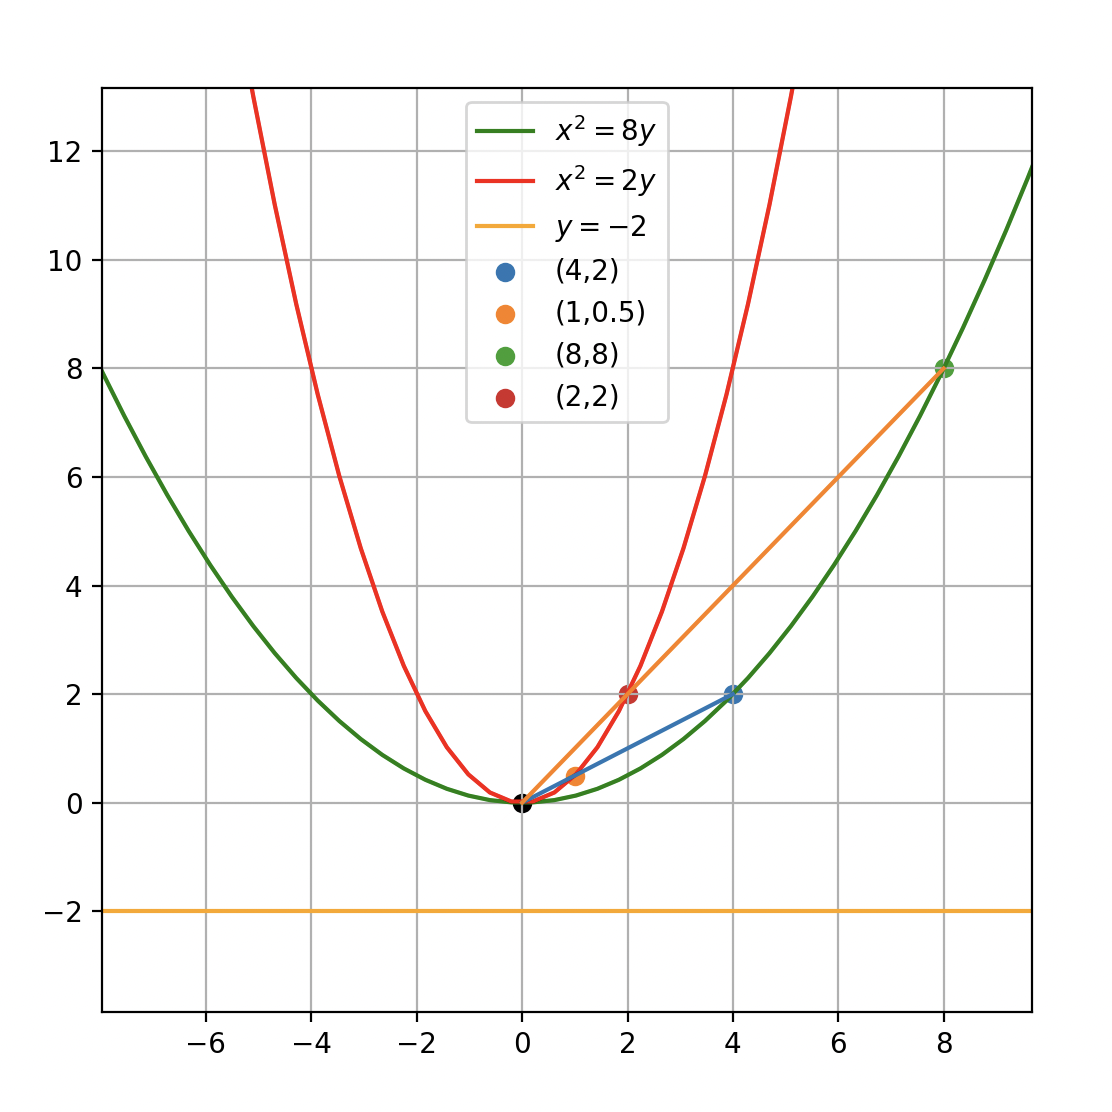
\includegraphics[width=0.6\columnwidth]{847.png}
    \caption{Plot}
    \label{fig:placeholder}
\end{figure}
\end{frame}

\end{document}